\documentclass{beamer}

% Beamer style
%\usetheme[secheader]{Madrid}
\usetheme{CambridgeUS}
\usecolortheme[rgb={0.65,0.15,0.25}]{structure}
%\usefonttheme[onlymath]{serif}
\beamertemplatenavigationsymbolsempty
%\AtBeginSubsection

% Packages
%\usepackage[french]{babel}
\usepackage[latin1]{inputenc}
\usepackage{color}
%\usepackage{dsfont, stmaryrd}
\usepackage{amsmath, amsfonts, amssymb}
\usepackage{epsfig}
\usepackage{url}
\usepackage{/home/robin/LATEX/astats}
%\usepackage[all]{xy}
\usepackage{graphicx}

% Commands
\definecolor{darkred}{rgb}{0.65,0.15,0.25}
\newcommand{\emphase}[1]{\textcolor{darkred}{#1}}
%\newcommand{\emphase}[1]{{#1}}
\newcommand{\paragraph}[1]{\textcolor{darkred}{#1}}
\newcommand{\refer}[1]{[\footnotesize{\textcolor{blue}{{\cite{#1}}}}]}
\newcommand{\Refer}[1]{[\textcolor{blue}{{\sl #1}}]}
\newcommand{\newblock}{}

% Symbols
\newcommand{\Abf}{{\bf A}}
\newcommand{\Beta}{\text{B}}
\newcommand{\Bcal}{\mathcal{B}}
\newcommand{\BIC}{\text{BIC}}
\newcommand{\Ccal}{\mathcal{C}}
\newcommand{\dd}{\text{~d}}
\newcommand{\dbf}{{\bf d}}
\newcommand{\Dcal}{\mathcal{D}}
\newcommand{\Esp}{\mathbb{E}}
\newcommand{\Ebf}{{\bf E}}
\newcommand{\Ecal}{\mathcal{E}}
\newcommand{\Gcal}{\mathcal{G}}
\newcommand{\Gam}{\mathcal{G}\text{am}}
\newcommand{\Ibb}{\mathbb{I}}
\newcommand{\Ibf}{{\bf I}}
\newcommand{\ICL}{\text{ICL}}
\newcommand{\Cov}{\mathbb{C}\text{ov}}
\newcommand{\Corr}{\mathbb{C}\text{orr}}
\newcommand{\Var}{\mathbb{V}}
\newcommand{\Vsf}{\mathsf{V}}
\newcommand{\pen}{\text{pen}}
\newcommand{\Fcal}{\mathcal{F}}
\newcommand{\Hbf}{{\bf H}}
\newcommand{\Hcal}{\mathcal{H}}
\newcommand{\Jcal}{\mathcal{J}}
\newcommand{\Kbf}{{\bf K}}
\newcommand{\Lcal}{\mathcal{L}}
\newcommand{\Mcal}{\mathcal{M}}
\newcommand{\mbf}{{\bf m}}
\newcommand{\mum}{\mu(\mbf)}
\newcommand{\Ncal}{\mathcal{N}}
\newcommand{\Nbf}{{\bf N}}
\newcommand{\Nm}{N(\mbf)}
\newcommand{\Ocal}{\mathcal{O}}
\newcommand{\Obf}{{\bf 0}}
\newcommand{\Omegas}{\underset{s}{\Omega}}
\newcommand{\Pbf}{{\bf P}}
\newcommand{\Pcal}{\mathcal{P}}
\newcommand{\Qcal}{\mathcal{Q}}
\newcommand{\Rbb}{\mathbb{R}}
\newcommand{\Rcal}{\mathcal{R}}
\newcommand{\sbf}{{\bf s}}
\newcommand{\Sbf}{{\bf S}}
\newcommand{\Scal}{\mathcal{S}}
\newcommand{\Ucal}{\mathcal{U}}
\newcommand{\Vcal}{\mathcal{V}}
\newcommand{\Tbf}{{\bf T}}
\newcommand{\ubf}{{\bf u}}
\newcommand{\Ubf}{{\bf U}}
\newcommand{\Wbf}{{\bf W}}
\newcommand{\xbf}{{\bf x}}
\newcommand{\Xbf}{{\bf X}}
\newcommand{\ybf}{{\bf y}}
\newcommand{\Ybf}{{\bf Y}}
\newcommand{\zbf}{{\bf z}}
\newcommand{\Zbf}{{\bf Z}}
\newcommand{\betabf}{\text{\mathversion{bold}{$\beta$}}}
\newcommand{\pibf}{\text{\mathversion{bold}{$\pi$}}}
\newcommand{\phibf}{\text{\mathversion{bold}{$\phi$}}}
\newcommand{\Sigmabf}{\text{\mathversion{bold}{$\Sigma$}}}
\newcommand{\gammabf}{\text{\mathversion{bold}{$\gamma$}}}
\newcommand{\mubf}{\text{\mathversion{bold}{$\mu$}}}
\newcommand{\nubf}{\text{\mathversion{bold}{$\nu$}}}
\newcommand{\Thetabf}{\text{\mathversion{bold}{$\Theta$}}}
\newcommand{\thetabf}{\text{\mathversion{bold}{$\theta$}}}
\newcommand{\BP}{\text{BP}}
\newcommand{\EM}{\text{EM}}
\newcommand{\VEM}{\text{VEM}}
\newcommand{\VBEM}{\text{VBEM}}
\newcommand{\cst}{\text{cst}}
\newcommand{\obs}{\text{obs}}
\newcommand{\ra}{\emphase{\mathversion{bold}{$\rightarrow$}~}}
\newcommand{\QZ}{Q_{\Zbf}}
\newcommand{\Qt}{Q_{\thetabf}}
%\newcommand{\transp}{\text{{\tiny $\top$}}}
\newcommand{\transp}{\text{{\tiny \mathversion{bold}{$\top$}}}}

% Directory
\newcommand{\figmixt}{/home/robin/ENSEIGN/COURS/MELANGE}
\newcommand{\figbma}{/home/robin/RECHERCHE/RUPTURES/MELANGE/Exemples/Grippe}
\newcommand{\fignet}{../FIGURES}
\newcommand{\figeco}{/home/robin/RECHERCHE/ECOLOGIE/EXPOSES/FIGURES}
%\newcommand{\figmotif}{/home/robin/RECHERCHE/RESEAUX/Motifs/FIGURES}


%--------------------------------------------------------------------
%--------------------------------------------------------------------

%--------------------------------------------------------------------
%--------------------------------------------------------------------
\begin{document}
%--------------------------------------------------------------------
%--------------------------------------------------------------------

%--------------------------------------------------------------------
\frame{\frametitle{Stochastic Block Model (SBM)}

  \begin{tabular}{cc}
    \hspace{-.5cm}
    \begin{tabular}{p{.5\textwidth}}
%      \onslide+<1->{
	\paragraph{A mixture model for random graphs.}%}
%      \onslide+<2->{
	\begin{itemize}
        \item Consider $n$ nodes ($i = 1..n$); \\ ~ %} 
%        \onslide+<3->{
        \item $Z_i = $ unobserved label of node $i$:
          $$
          \{Z_i\} \text{ i.i.d. } \sim \Mcal(1; \pi)
          $$
          $\pi = (\pi_1, ... \pi_K)$; \\ ~ %} 
%        \onslide+<4->{
        \item Edge $Y_{ij}$ depends on the labels:
          $\{Y_{ij}\}$ independent given $\{Z_i\}$,
          $$
          (Y_{ij}) \sim \Bcal(\gamma_{Z_i, Z_j})
          $$%}
      \end{itemize}
    \end{tabular}
    & 
    \hspace{-.5cm}
    \begin{tabular}{p{.5\textwidth}}
      \vspace{1cm}
      \begin{overprint}
        \onslide<2>
        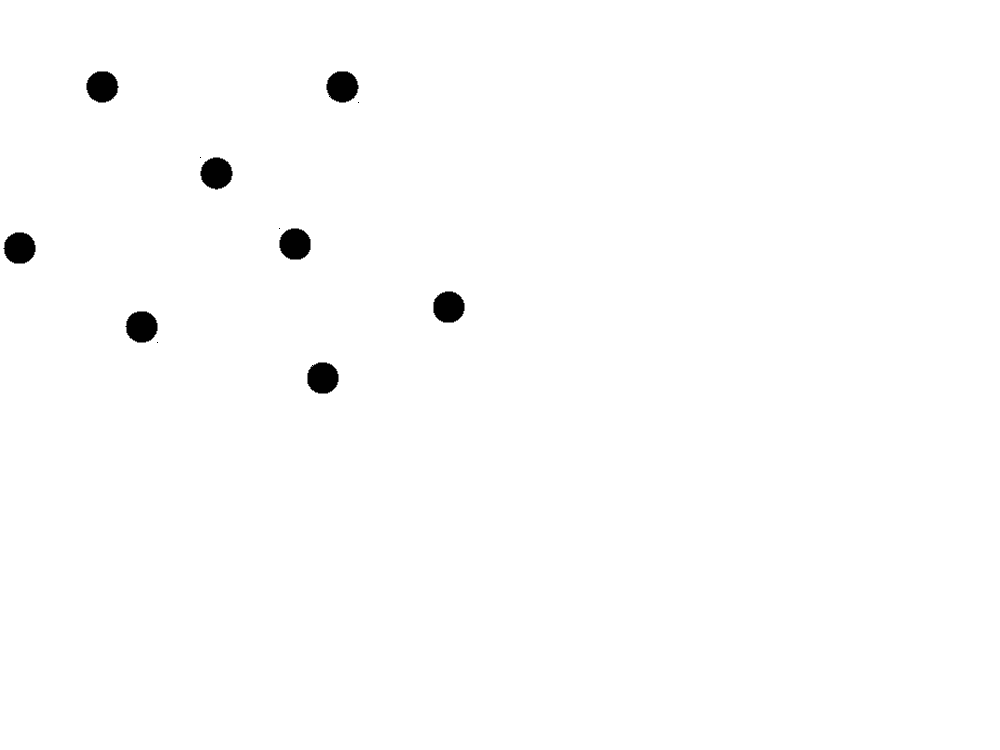
\includegraphics[width=.75\textwidth]{\fignet/FigSBM-Model-1}    
        \onslide<3>
        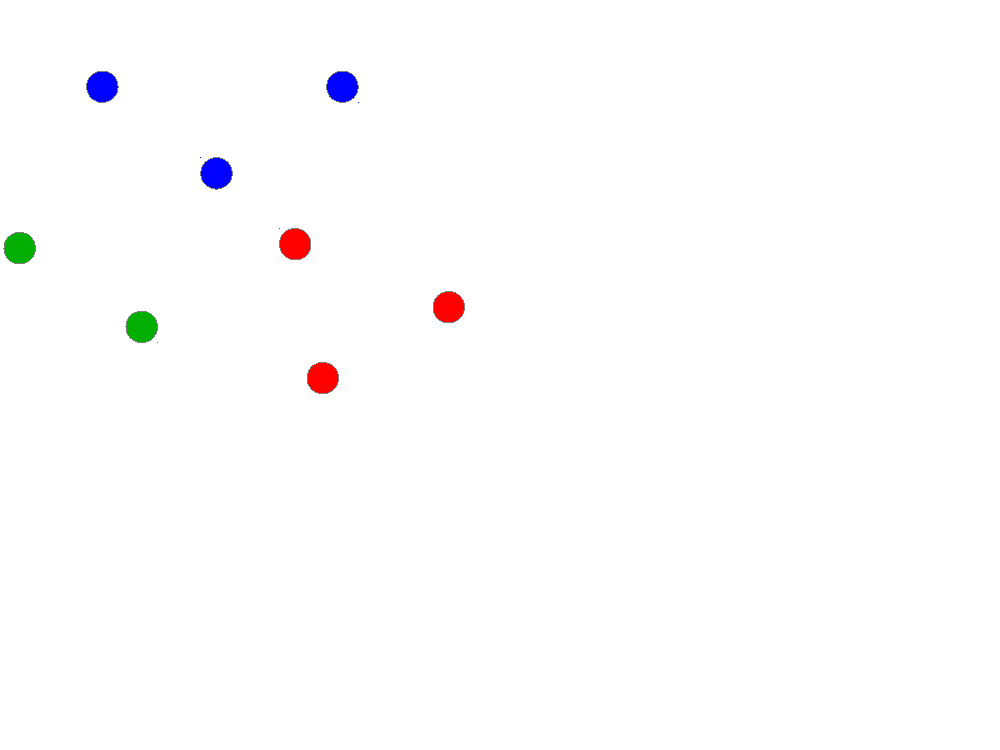
\includegraphics[width=.75\textwidth]{\fignet/FigSBM-Model-2}    
        \onslide<4>
        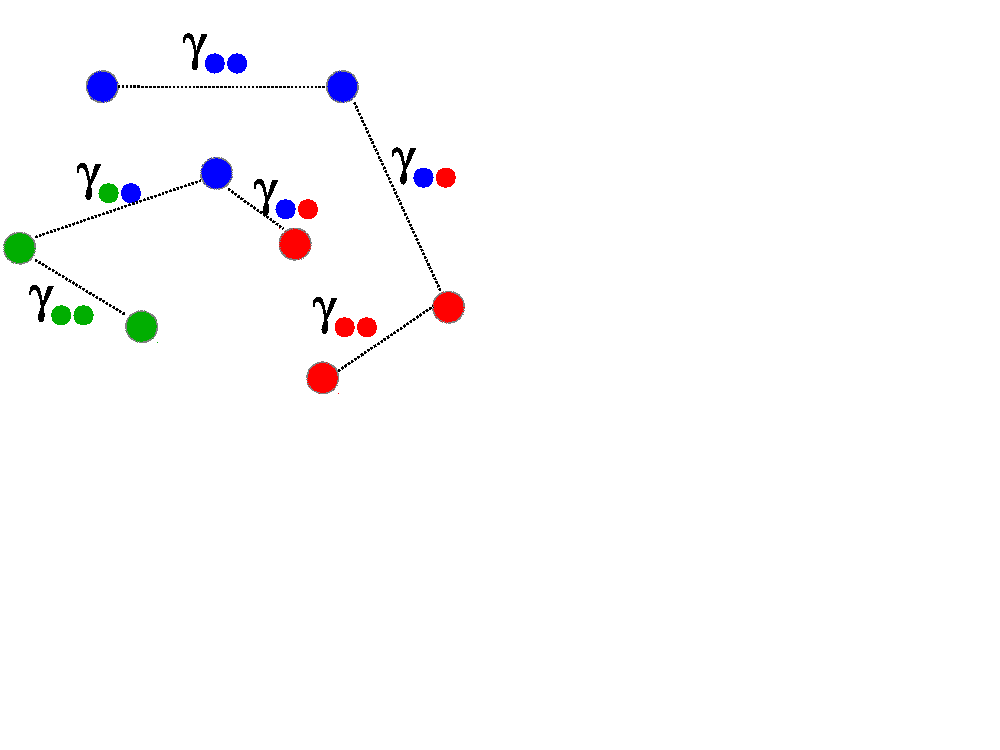
\includegraphics[width=.75\textwidth]{\fignet/FigSBM-Model-3}    
        \onslide<5>
%        \epsfig{file = \fignet/FigSBM-Model-4.eps,
%        width=.75\textwidth, clip=}    
%        \onslide<6>
        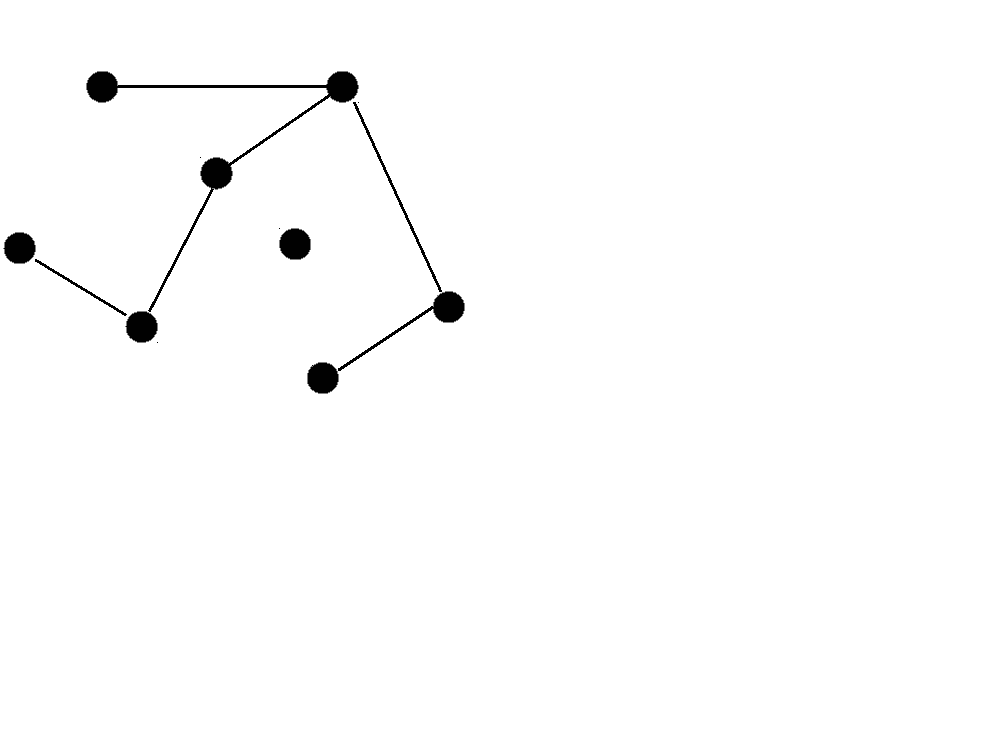
\includegraphics[width=.75\textwidth]{\fignet/FigSBM-Model-5}    
      \end{overprint}
    \end{tabular}
  \end{tabular}
  }

%-------------------------------------------------------------------- 
\frame{ \frametitle{SBM analysis of {\sl E. coli} operon networks}

  \vspace{-0.5cm}
  \hspace{-0.5cm}
  \begin{tabular}{cc}         
    \begin{tabular}{p{0.45\textwidth}}
%       \onslide+<1->{
	%\vspace{-1cm}
        \includegraphics[width=.45\textwidth]{\fignet/im_EcoliVEM_2} \\
          %~\\
%          \refer{PMD09}
%         }
    \end{tabular}
    &
    \begin{tabular}{p{0.45\textwidth}}
%     \onslide+<2->{
      %\vspace{-.3cm}
      \paragraph{Meta-graph representation.} \\
      %\vspace{-.5cm}
      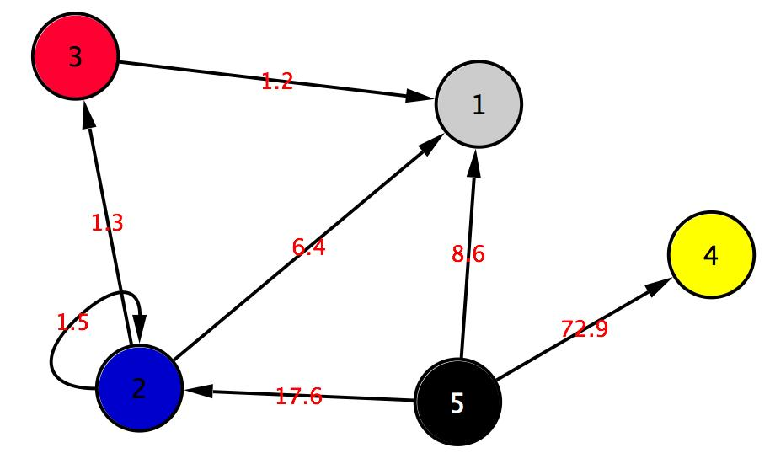
\includegraphics[width=.35\textwidth]{\fignet/VEMmetagraphe}  \\
%     }
%     \onslide+<3->{
      \vspace{-.3cm}
      \paragraph{Parameter estimates.} $K = 5$     \\
      \includegraphics[width=.35\textwidth]{../FIGURES/im-pi1BVEM}\\        
      \includegraphics[width=.35\textwidth]{../FIGURES/im-pi2BVEM}\\
      \includegraphics[width=.35\textwidth]{../FIGURES/im-pi3BVEM}\\
      \includegraphics[width=.35\textwidth]{../FIGURES/im-pi4BVEM}\\
      \includegraphics[width=.35\textwidth]{../FIGURES/im-pi5BVEM}\\
      \hline 
      \includegraphics[width=.35\textwidth]{../FIGURES/im-alphaBVEM}\\
%     }
    \end{tabular}
  \end{tabular}
  }

%--------------------------------------------------------------------
\frame{ \frametitle{{\VBEM} Credibility intervals and convergence}

  \paragraph{Actual level as a function of $n$:}   $\pi_1$: $+$,
  $\gamma_{11}$: \textcolor{red}{$\triangle$}, $\gamma_{12}$:
  \textcolor{blue}{$\circ$}, $\gamma_{22}$: \textcolor{green}{$\bullet$}
  $$
  \includegraphics[width=1\textwidth]{../FIGURES/im-ICQ2-2-new} 
  $$

  \emphase{Width of the posterior credibility intervals.}
  {$\pi_1$}, \textcolor{red}{$\gamma_{11}$},
  \textcolor{blue}{$\gamma_{12}$}, \textcolor{green}{$\gamma_{22}$}
  \\
  \includegraphics[width=1\textwidth]{../FIGURES/im-ICQ2-3} \\

 }

%-------------------------------------------------------------------- 
\frame{ \frametitle{Concentration of the degree distribution} 

  \begin{overprint}
   \onslide<1>
   \paragraph{$n = 100$.}
  $$
  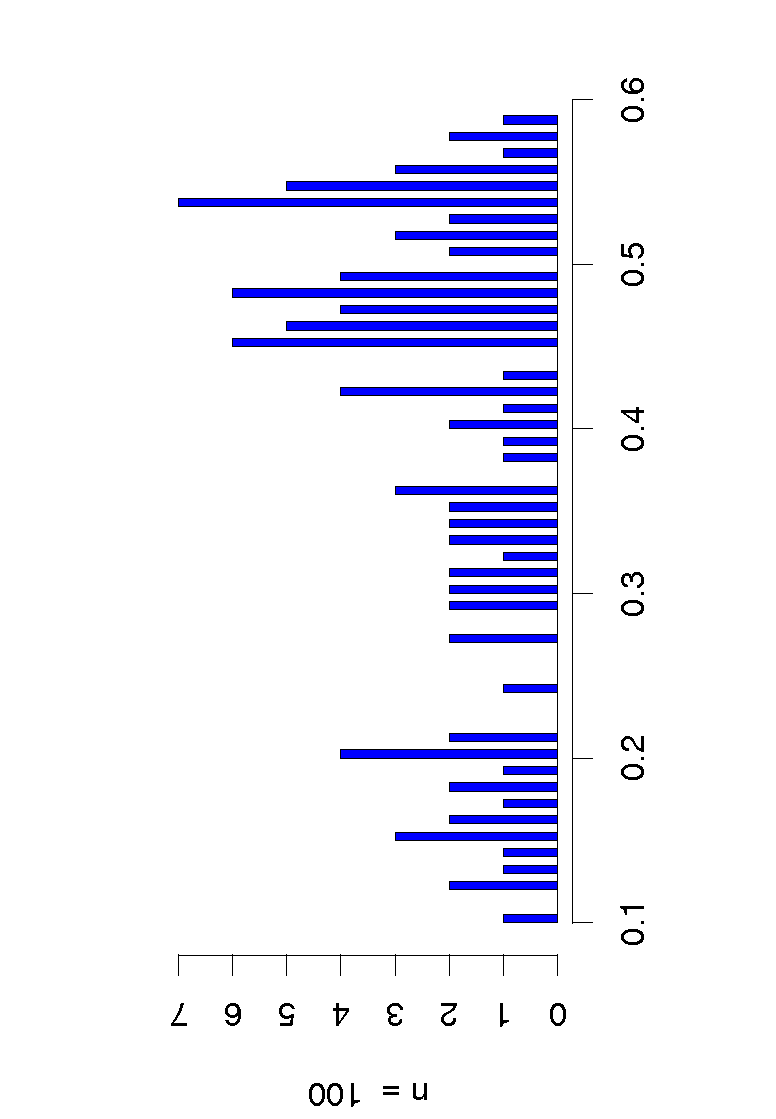
\includegraphics[width=.5\textwidth, angle=270]{\fignet/ConcentrBinom-n100}
  $$
   \onslide<2>
   \paragraph{$n = 1000$.}
  $$
  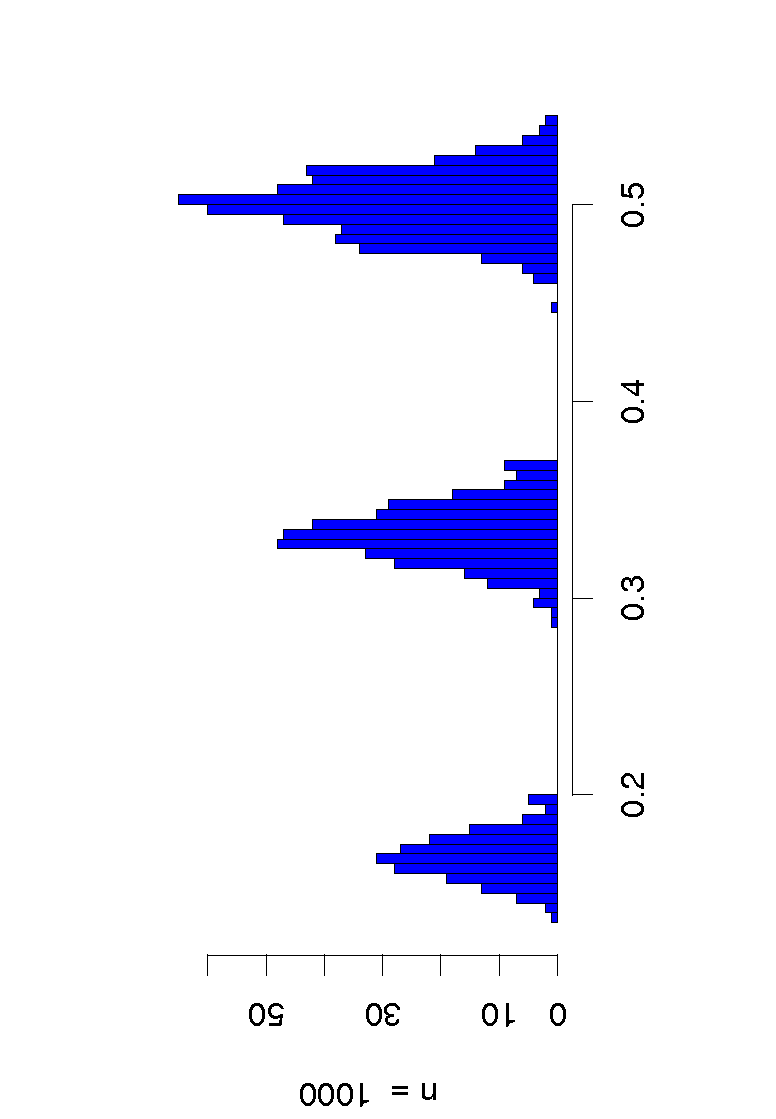
\includegraphics[width=.5\textwidth, angle=270]{\fignet/ConcentrBinom-n1000}
  $$
   \onslide<3>
   \paragraph{$n = 10000$.}
  $$
  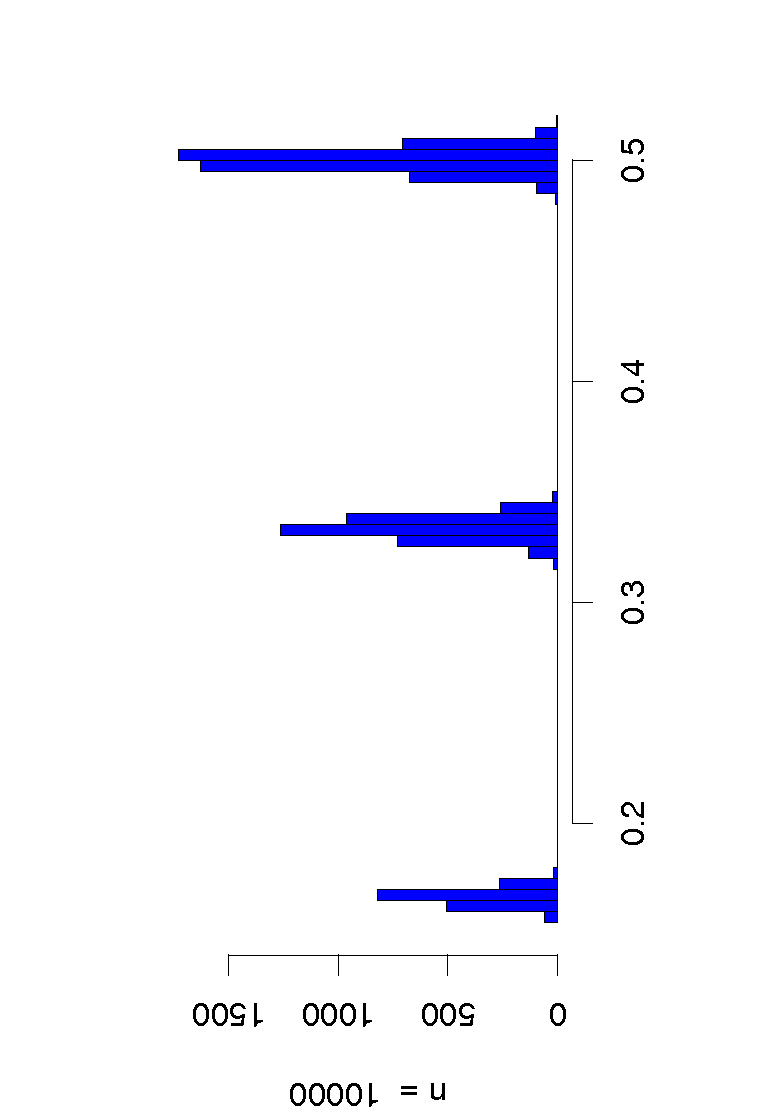
\includegraphics[width=.5\textwidth, angle=270]{\fignet/ConcentrBinom-n10000}
  $$
  \end{overprint}
  }
  

%--------------------------------------------------------------------
\frame{ \frametitle{Tree interaction network}
  \begin{tabular}{cc}
    \hspace{-.5cm}
    \begin{tabular}{p{.4\textwidth}}
      \paragraph{Data:} $n = 51$ tree species, \\
      $Y_{ij}=$ number of shared parasites. % (\refer{VPD08}).

%      \onslide+<2->{
        \bigskip
        \paragraph{Model:}
        $$
        Y_{ij} \sim \Pcal(\lambda_{k\ell}),
        $$
        $\lambda_{k\ell} =$ mean number of shared parasites.
        
        \bigskip
        \paragraph{Results:} ICL selects $K=7$ groups%}
%      \onslide+<3->{
        that are \emphase{strongly related with phylums}. 
%        }
      \end{tabular}
    & 
    \hspace{-.75cm}
    \begin{tabular}{c}
%      \onslide+<2->{
        {\tiny
          \begin{tabular}{c|ccccccc}
            $\widehat{\lambda}_{k\ell}$ & T1 & T2 & T3 & T4 & T5 & T6 &
            T7 \\ 
            \hline
            T1 & 14.46 & 4.19 & 5.99 & 7.67 & 2.44 & 0.13 & 1.43 \\
            T2 &  & 14.13 & 0.68 & 2.79 & 4.84 & 0.53 & 1.54 \\
            T3 &  &  & 3.19 & 4.10 & 0.66 & 0.02 & 0.69 \\
            T4 &  &  &  & 7.42 & 2.57 & 0.04 & 1.05 \\
            T5 &  &  &  &  & 3.64 & 0.23 & 0.83 \\
            T6 &  &  &  &  &  & 0.04 & 0.06 \\
            T7 &  &  &  &  &  &  & 0.27 \\
            \hline \hline
            $\widehat{\pi}_k$ & 7.8 & 7.8 & 13.7 & 13.7 & 15.7 & 19.6 &
            21.6  
          \end{tabular}
          }\\
%        }
%      \onslide+<3->{
        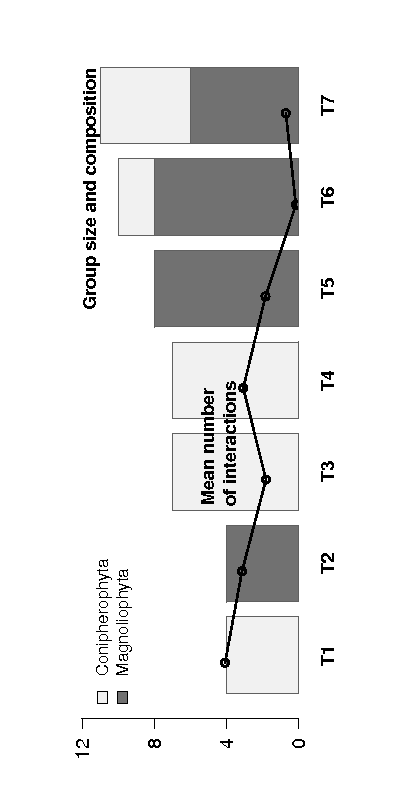
\includegraphics[width=.6\textheight, height=.6\textwidth, angle=270]{\fignet/MRV10_AoAS_Q7_group}
%        }
    \end{tabular}
  \end{tabular}
  }

%--------------------------------------------------------------------
\frame{ \frametitle{Accounting for the taxonomic distance $d_{ij}$}
  \begin{tabular}{cc}
    \hspace{-.5cm}
    \begin{tabular}{p{.4\textwidth}}
      \paragraph{Model:}
      $$
      Y_{ij} \sim \Pcal[\lambda_{k\ell} \; \emphase{\exp(\beta d_{ij})}].
      $$

      \bigskip%\pause
      \paragraph{Results:} $\widehat{\beta} = -0.317$. \\
      \ra for $\overline{d} = 3.82$, 
      $$
      e^{\widehat{\beta}\overline{d}} = .298
      $$
      \ra The mean number of shared parasites \emphase{decreases as
        the distance increases}.
      %\pause
    \end{tabular}
    & 
    %\hspace{-.75cm}
    \begin{tabular}{c}
      {\tiny
        \begin{tabular}{c|cccc}
          $\widehat{\lambda}_{k\ell}$ & T'1 & T'2 & T'3 & T'4 \\ 
          \hline
          T'1 & 0.75 & 2.46 & 0.40 & 3.77 \\
          T'2 &  & 4.30 & 0.52 & 8.77 \\ 
          T'3 &  &  & 0.080 & 1.05 \\ 
          T'4 &  &  &  & 14.22 \\
          \hline \hline
          $\widehat{\pi}_k$ & 17.7 & 21.5 & 23.5 & 37.3 \\
          \hline \hline
          $\widehat{\beta}$ & \multicolumn{4}{c}{-0.317}
        \end{tabular}
        } \\ 
      %\pause
      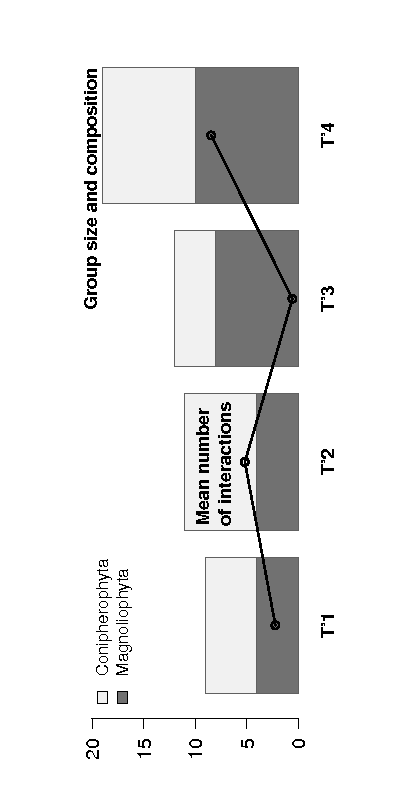
\includegraphics[width=.5\textheight, height=.5\textwidth, angle=270]{\fignet/MRV10_AoAS_Q4_group}
    \end{tabular}
  \end{tabular}
  
%   \ra Groups are no longer associated with the phylogenetic
%   structure. \\
%   \ra Mixture $=$ \emphase{residual heterogeneity} of the regression.
  }

%--------------------------------------------------------------------
\frame{ \frametitle{Estimation of the $W$ graphon}

  \paragraph{French political blogosphere.} $\widehat{W}(u, v) = \Esp(\gamma(u, v) | Y)$
  $$
  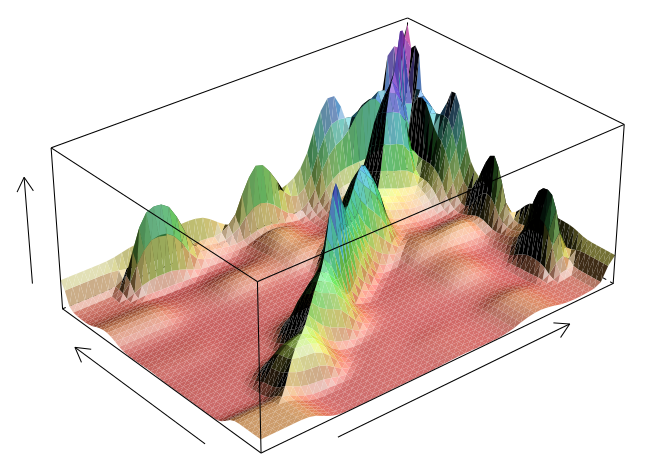
\includegraphics[width=.65\textwidth]{../FIGURES/wireframe}
  $$
  Motif probability can be estimated as well as $\widehat{\mu}(m) = \Esp(\mu(m) | Y)$.
}

%--------------------------------------------------------------------
%--------------------------------------------------------------------
\end{document}
%--------------------------------------------------------------------
%--------------------------------------------------------------------

  \begin{tabular}{cc}
    \hspace{-.5cm}
    \begin{tabular}{p{.5\textwidth}}
    \end{tabular}
    & 
    \hspace{-.5cm}
    \begin{tabular}{p{.5\textwidth}}
    \end{tabular}
  \end{tabular}
